\documentclass[handout]{beamer}
%\documentclass[xcolor=pst]{beamer}
%\usepackage[spanish]{babel}
\usepackage[utf8]{inputenc}

\usepackage{amssymb,amsmath}
\usepackage{bbm}
\usepackage{graphicx}
%\usepackage[pdf]{pstricks}
\usepackage{colortbl}
\definecolor{fucsia}{rgb}{1,0,1}
%\usepackage[Q=yes]{examplep}

\newcounter{savedenum}
\newcommand*{\saveenum}{\setcounter{savedenum}{\theenumi}}
\newcommand*{\resume}{\setcounter{enumi}{\thesavedenum}}

%\usepackage{default}
\usetheme{Madrid}

%\setbeamertemplate{caption}[numbered]


\title[L-Shape Selection]{A heuristic algorithm to select genes potentially regulated by methylation}
\author[Alex S\'anchez]{Alex S\'anchez, Berta Mir\'o, Francesc Carmona, \\
	Sarah Bazzoco and Diego Arango del Corro}
\date[]{July 09, 2018}

\begin{document}
\begin{frame}
	
\begin{scriptsize}
\begin{center}
  \emph{ XXII International Biometric Conference}
\end{center}
\end{scriptsize}

\titlepage

\begin{columns}
   \column{0.7\textwidth}
   \scriptsize
   Genetics, Microbiology and Statistics Department \\ 
   \textbf{Facultad de Biología, Universitat de Barcelona}\\
   Statistics and Bioinformatics Unit (UEB)\\
   Department Molecular Oncology-CIBBIM \\ 
   \textbf{Vall Hebron Institut de Recerca}

  \hfill\column{0.3\textwidth}
  
\includegraphics[height=1cm]{images/alllogos.png}
% 
\includegraphics[height=0.5cm]{images/VHIR_fonstransp.png}
\end{columns}

\end{frame}


\begin{frame}
\frametitle{Table of Contents}
\tableofcontents
\end{frame}

\section{Introduction / Motivation}

\subsection{Genome-wide analysis of colorectal cancer}

\begin{frame}
	\frametitle{Genome-wide analysis of colorectal cancer}
	  \begin{itemize}
	  	\item CRC is a serious public health problem (2.M diagnosed/year) but the number of therapies available is smaller than in other cancer types.
	  	\item Researcher's interest: identification of biomarkers for chemotherapy sensitivity in colorectal cancer (CRC).
	  	%\item The study analyzed a panel of 30--45 cell lines derived from colorectal tumors characterized by increasing sensitivity to several chemotherapy drugs (Irinotecan, Cetuximab, Oxaliplatin).
	  	\item The researchers' approach was to look for \textit{genes regulated by methylation} which could be considered possible therapeutic targets.
	  	\end{itemize}
\end{frame}

\begin{frame}
	\frametitle{Methylation}
	\begin{itemize}
		\item Methylation of CpG dinucleotides in the promoter of genes
		involved in the oncogenic process has been shown to be a key process
		contributing to tumor initiation and/or progression.
		\item Essentially (and especially in cancer) methylation acts by inhibiting gene expression that
		is,\emph{ the more methylated is a gene the more repressed is its expression}
		\begin{center}
			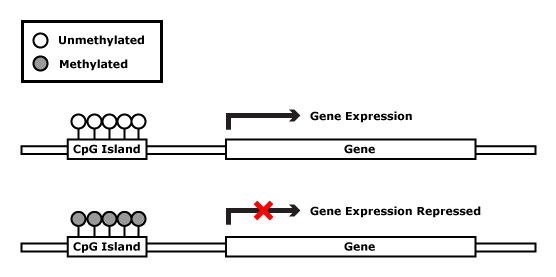
\includegraphics[width=0.7\textwidth]{./images/methylationAction1.png}
		\end{center}
	\end{itemize}
\end{frame}


\begin{frame}[fragile]\frametitle{Methylation and gene expression}
	\begin{itemize}
		\item Although the relation between methylation and gene expression is probably continuous ("\emph{the more...the less...}"),
		\begin{center}
			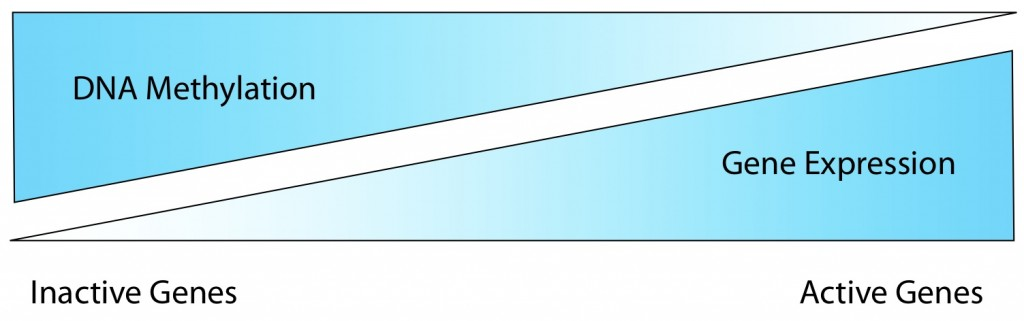
\includegraphics[width=0.7\textwidth]{./images/DNA-Methylation-and-Gene-Expression-Relationship.jpg}
		\end{center}
		\item methylation is, in practice, seen as a dual phenomenon
		\begin{itemize}
			\item A methylated gene is ``off''
			\item An unmethylated gene is ``on''
		\end{itemize}
		\item Practical problem: \textbf{\emph{at which methylation level a gene is seen as ``methylated'' (is it ``turned off'')?}}
	\end{itemize}
	
\end{frame}


\begin{frame}{Patterns of (negative) association}
	\begin{itemize}
		\item Considering the relation between methylation and expression in cancer (the higher methylation the lower the expression...)
		\item leads to expecting that scatterplots depicting the relation between methylation and expression show a negative correlation.
		\item This is usually the case and, indeed, \textit{genes known to be regulated by methylation often show \textbf{an L-shape pattern} in these plots}.
	\end{itemize}
	\begin{center}
		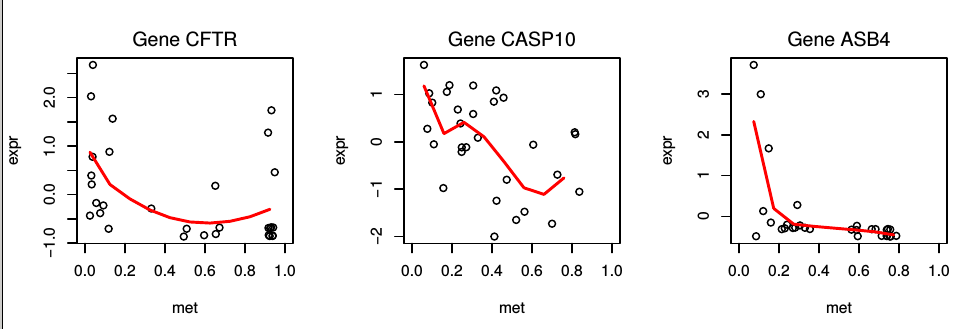
\includegraphics[width=0.7\textwidth]{./images/Lshapes1.png}
	\end{center}
\end{frame}

\begin{frame}{Selecting genes by mining scatterplots}
	\begin{itemize}
		\item Assuming the relation described above is true...
		\item Finding genes regulated by methylation is equivalent to finding genes whose methylation--expression scatterplot has an L--shape.
		\item There is a scatterplot \emph{per} gene and thousands of genes:\\ {\emph{Automatic methods for selecting interesting genes through their scatterplots are required}}.
		\item There exist methods  that add on the correlation coefficient but they are not very successful.
	\end{itemize}
\end{frame}


\subsection{Objectives}

\begin{frame}
	\frametitle{Objectives}
	
The main objectives of this work are:
\begin{enumerate}
	
	\item To introduce a new method to select genes showing an L-shape
	\item To compare it with previously available methods, 
	\item To apply the selected methods on a specific CRC dataset and validate the findings based on their biological relevance.
	
\end{enumerate}

\end{frame}

\section{Methods for selecting L-shaped patterns}


\frame<0>{
	\frametitle{Naïve method}
\begin{columns}%
	\begin{column}[t]{0.5\textwidth}%

		\begin{itemize}
			\item Simplest approach: Call a gene potentially regulated by methylation if a negative correlation between expression and methylation is observed.
			\item Most prevalent approach. (eg: Bioc. \texttt{MethylMix} package).
			\item Drawbacks:
			\begin{itemize}
				\item Lack of power.
				\item Easy to miss ``sharp'' L shapes.
			\end{itemize}
		\end{itemize}
		
	\end{column}
	\begin{column}[t]{0.5\textwidth}%
		\begin{center}
			\begin{figure}[h]          
				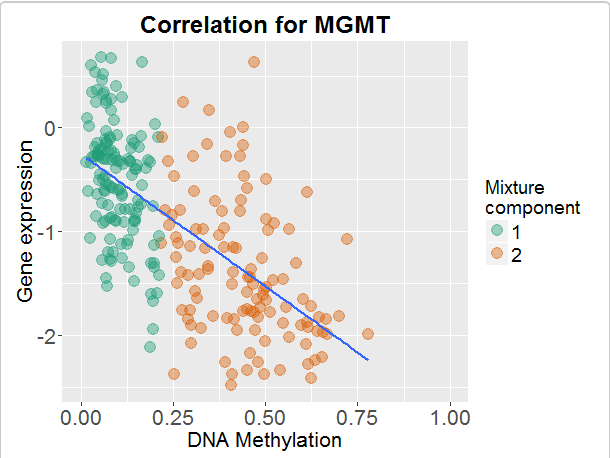
\includegraphics[width=0.9\textwidth]{images/corrInMethylMix.png}
			\end{figure}
		\end{center}
	\end{column}
\end{columns}
}



\frame<0>{
	\frametitle{Conditional Mutual Information}
\begin{itemize}
	\item Following \cite{Liu:2012} in order to determine whether methylation $X$ and expression $Y$ of a gene exhibit an L--shape, the conditional Mutual Information $cMI(t)$ for different choices of threshold $t$ is computed.
	\[
	\mathit{cMI}(t)=I(X,Y|X>t)P(X>t) + I(X,Y|X\le t)P(X\le t)
	\]
	\item If the relation between methylation and expression shows an L-shape  as $t$ moves from 0 to 1, $\mathit{cMI}(t)$ first decreases and then increases, its value approaching zero when $t$ coincides with the reflection point. 
\begin{center}
	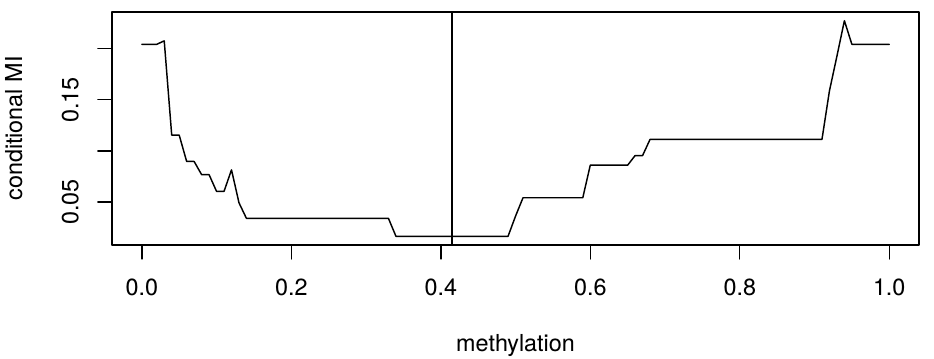
\includegraphics[height=2.5cm]{./images/cMI-methylation.png}
\end{center}
	\item Genes whose cMI go below a threshold can be considered L-shaped.
\end{itemize}
}

\begin{frame}
\frametitle{Some previously applied methods}

	\begin{itemize}
		\item Naive method: Call regulated by methylation genes depictinhg negative correlation between expression and methylation
		\item Study variation of conditional mutual information along different methylation values.\cite{Liu:2012}.
		\item Use regression splines to fit a curve to the scatterplot and use clustering to group patterns. \cite{Sanchez:2017}.
		\item Analyze scatterplots characteristics with Tukey's Scagnostics method \cite{Wilkinson:2017}
	\end{itemize}
\end{frame}

\subsection{A new algorithm}

\begin{frame}
	\frametitle{What is an L-shape, whatsoever}
\begin{columns}%
	\begin{column}[t]{0.5\textwidth}%
		
		\begin{itemize}
			\item After trying different approaches to detect L-shapes, one  comes back to a naive approach like 
			\item \emph{``L-shaped'' genes should show an L shape in the scatterplot}; 
				\begin{itemize}
					\item  The more L-shaped a scatterplot the more its values scatter near the vertical and horizontal axes,
					\item The more these values move away move from these positions the least L-shaped the gene is.
				\end{itemize}
		\end{itemize}
		
	\end{column}
	\begin{column}[t]{0.5\textwidth}%
		\begin{center}
			\begin{figure}[h]          
				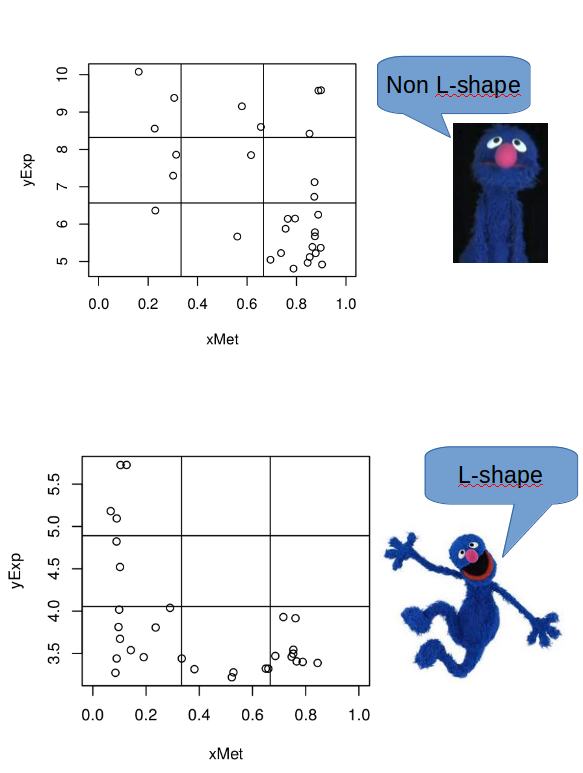
\includegraphics[width=\textwidth]{images/LshapeNonLshape.png}
			\end{figure}
		\end{center}
	\end{column}
\end{columns}	
\end{frame}

\begin{frame}
	\frametitle{A weighting system}
	\begin{enumerate}
		\item Overimpose a $3\times 3$ grid on the scatterplot.
		\item Classify the scatterplot as \textbf{``L'' or ``non-L''} based on a small set of conditions:
		\begin{enumerate}
			\item There must be a \emph{minimum} number of points in the upper-left (cell (1,1)) and lower right (cell (3,3)) corners of the grid.
			\item There must be a \emph{maximum} number of points in the upper right (cell (1,3)) because points there mean hypermethylation and hyperexpression which is the opposite of what we are looking for.
			\item We will usually \emph{not require to have a minimum of points in cell (3,1)} unless we are really willing to have an L-shape (in our setting we will also be happy tho recover diagonals, which also reflect a negative correlation!).
		\end{enumerate}
	\end{enumerate}
{
\begin{equation*}
\mathbbm{1}_L(X) = \bigwedge_{i,j} X \circ C \circ \left( mMP \times \sum_{i,j}x_{ij}\right),
\end{equation*}
}

\end{frame}

\begin{frame}
	\frametitle{A scoring system}
		\begin{enumerate}
			\item Score points on each subgrid in such a way that
			\begin{enumerate}
				\item Points in permitted regions (left-outer margin, i.e. cells: (1,1), (2,2), (3,1), (3,2), (3,3)) score positively if the scatterplot has been classified as L or zero if it has been classified as non-L.
				\item Points in non-desired regions (outer band. i.e. cells (1,2), (1,3), (2,3)) score negatively in all cases.
				\item Some regions may be declared neutral and not-score, such as cell (2,2).
			\end{enumerate}
			{
			\begin{equation*}
			S(X) = W_L \circ X \times \mathbbm{1}_L(X) + W_{L^C} \circ X \times \mathbbm{1}_{L^c}(X),
			\end{equation*}
		    }
			\item Use cross-validation to tune scoring parameters (\emph{if a set of positive and negative L-shaped genes is available}).
		\end{enumerate}
	

\end{frame}



\begin{frame}
	\frametitle{An example}

\begin{columns}%
	\begin{column}[t]{0.4\textwidth}%	

\begin{enumerate}

\item Min-Max Counts
$$
mMP =\bigl(\begin{smallmatrix}
	10 & 20 & 0\\ 
	5 & 0 & 20\\ 
	0 & 5 & 5
\end{smallmatrix}\bigr)
$$

\item Matrix of weights for TRUE L scatterplots
$$
W_{TRUE-L} =\bigl(\begin{smallmatrix}
2 & -2 & -25\\ 
1 & 0 & -2\\ 
1 & 1 & 2
\end{smallmatrix}\bigr)
$$

\item Matrix of weights for FALSE L scatterplots
$$
W_{FALSE-L} =\bigl(\begin{smallmatrix}
0 & -2 & -25\\ 
0 & 0 & -2\\ 
0 & 0 & 0
\end{smallmatrix}\bigr)
$$

\end{enumerate}

	\end{column}
	\begin{column}[t]{0.6\textwidth}%
		\bigskip
		\begin{center}
			\begin{figure}[h]          
				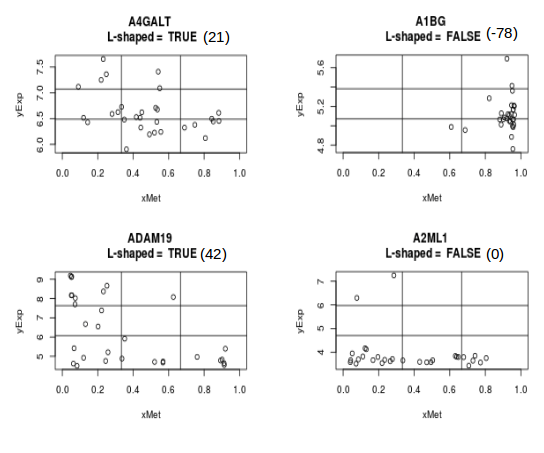
\includegraphics[width=\textwidth]{images/LshapeAndNonLshapeScored}
			\end{figure}
		\end{center}
	\end{column}
\end{columns}	
	
\end{frame}

\section{Results and Applications}

\begin{frame}
	\frametitle{Data for the comparisons}
	\begin{itemize}
		\item The methods have been tested using three real and one simulated dataset.
		\item Distinct datasets were generated by similar but not identical technologies.
		\item Genes non common to the three datasets were removed from the analysis
	\end{itemize}
\begin{table}[]
	\begin{tabular}{|l|l|c|c|l|l|}
		\hline
		\textit{Name} & \textit{Source} & \multicolumn{1}{l|}{\textit{Genes}} & \multicolumn{1}{l|}{\textit{Samples}} & \textit{Arrays}   & \textit{Methylation} \\ \hline
		\textbf{TCGA} & Nature 2012     & 1788                                & 223                                   &                   &                      \\ \hline
		\textbf{GEO}  & GSE25070        & 1191                                & 25                                    & Bead & 25K       \\ \hline
		\textbf{DA}   & Reseracher's    & 11359                               & 30                                    & Affy & 25k       \\ \hline
	\end{tabular}
\end{table}	
\end{frame}

\begin{frame}
	\frametitle{Results: Comparison between datasets}
\begin{center}
	\begin{figure}[h]          
		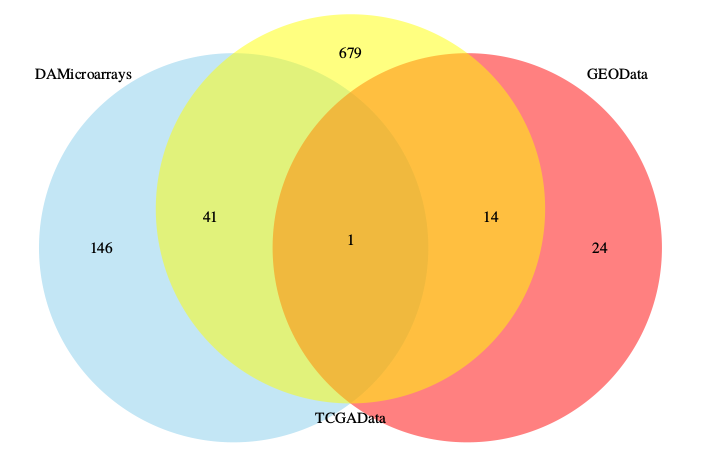
\includegraphics[height=0.8\textheight]{images/genesInCommonBetweenHEURISTICselections.png}
	\end{figure}
\end{center}
\end{frame}


\begin{frame}
	\frametitle{Results: Comparison between the methods}
\begin{center}
	\begin{figure}[h]          
		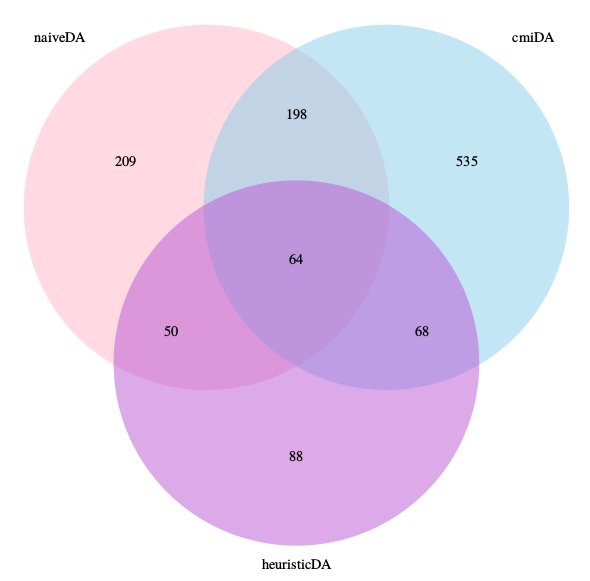
\includegraphics[height=0.8\textheight]{images/genesInCommonBetweenMethodsInDA.png}
	\end{figure}
\end{center}
\end{frame}

\frame[allowframebreaks]{\frametitle{Software}
	\begin{center}
		\begin{figure}[h]          
			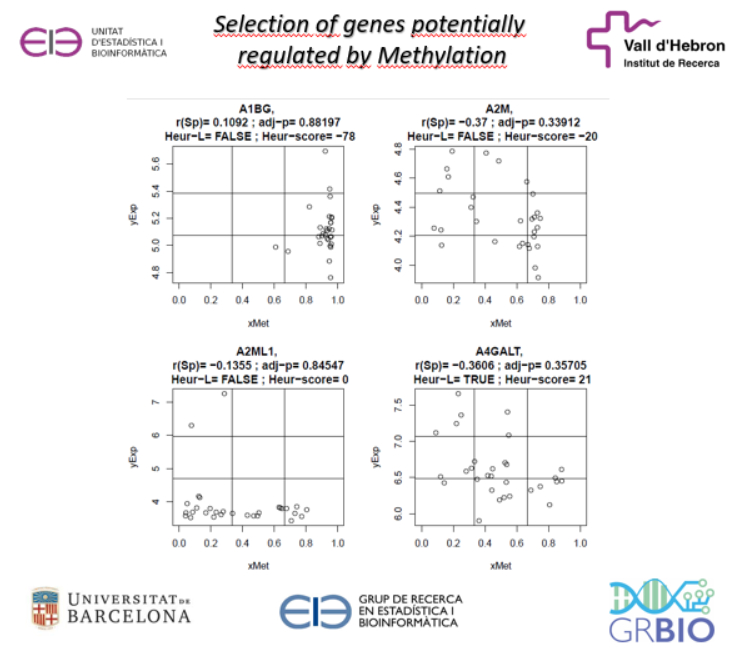
\includegraphics[height=0.8\textheight]{images/shinyApp1.png}
		\end{figure}
	\end{center}

	\begin{center}
	\begin{figure}[h]          
		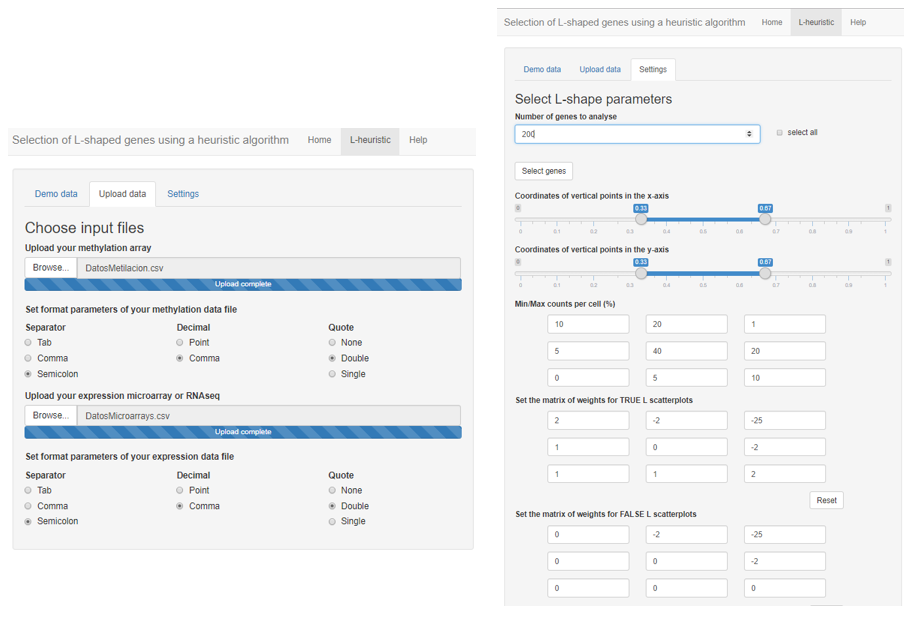
\includegraphics[height=0.8\textheight]{images/shinyApp2.png}
	\end{figure}
\end{center}

\begin{center}
	\begin{figure}[h]          
		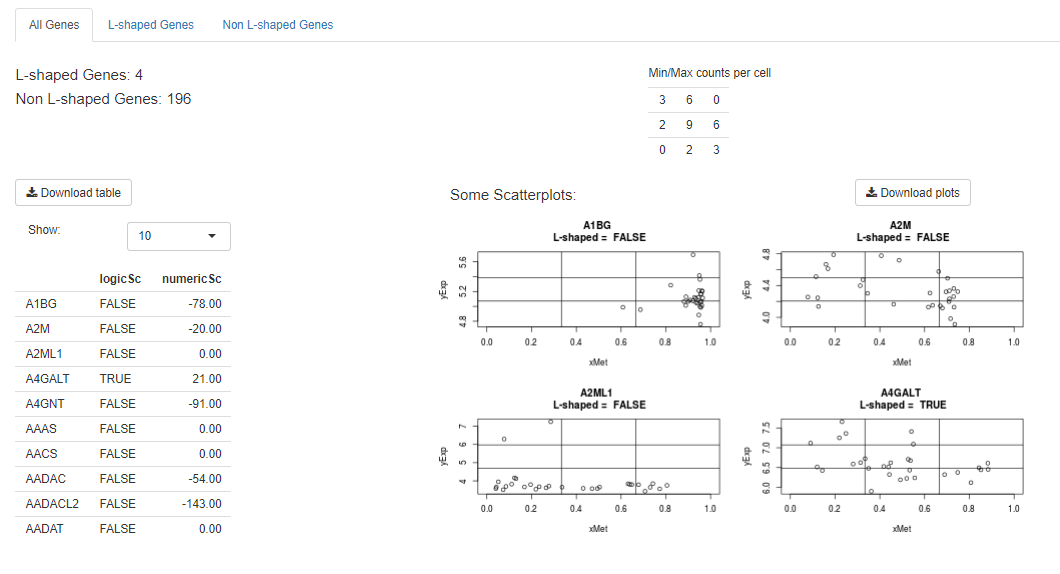
\includegraphics[width=0.8\textwidth]{images/shinyApp3.png}
	\end{figure}
\end{center}
}

\begin{frame}
\frametitle{Summary of results}
\end{frame}


\section{Discussion and conclusions}

\begin{frame}
	\frametitle{Limitations}
\end{frame}

\begin{frame}
	\frametitle{Conclusions}
\end{frame}



\begin{frame}{Acknowledgments}
	\begin{enumerate}
		\item My group ESTBIOINFO at the GME department at the University of Barcelona and the research group GRBio, led by Guadalupe Gómez.
		\item The Statistics and Bioinformatics Unit at Vall d'Hebron Institut de Recerca (VHIR).
		\item The Nanomedicine and Molecular Oncology group at VHIR, led by Dr. Diego Arango.
	\end{enumerate}
\end{frame}

\begin{frame}
	\begin{center}
		{\Huge
			Thanks for your attention!}
	\end{center}
	
	\begin{center}
		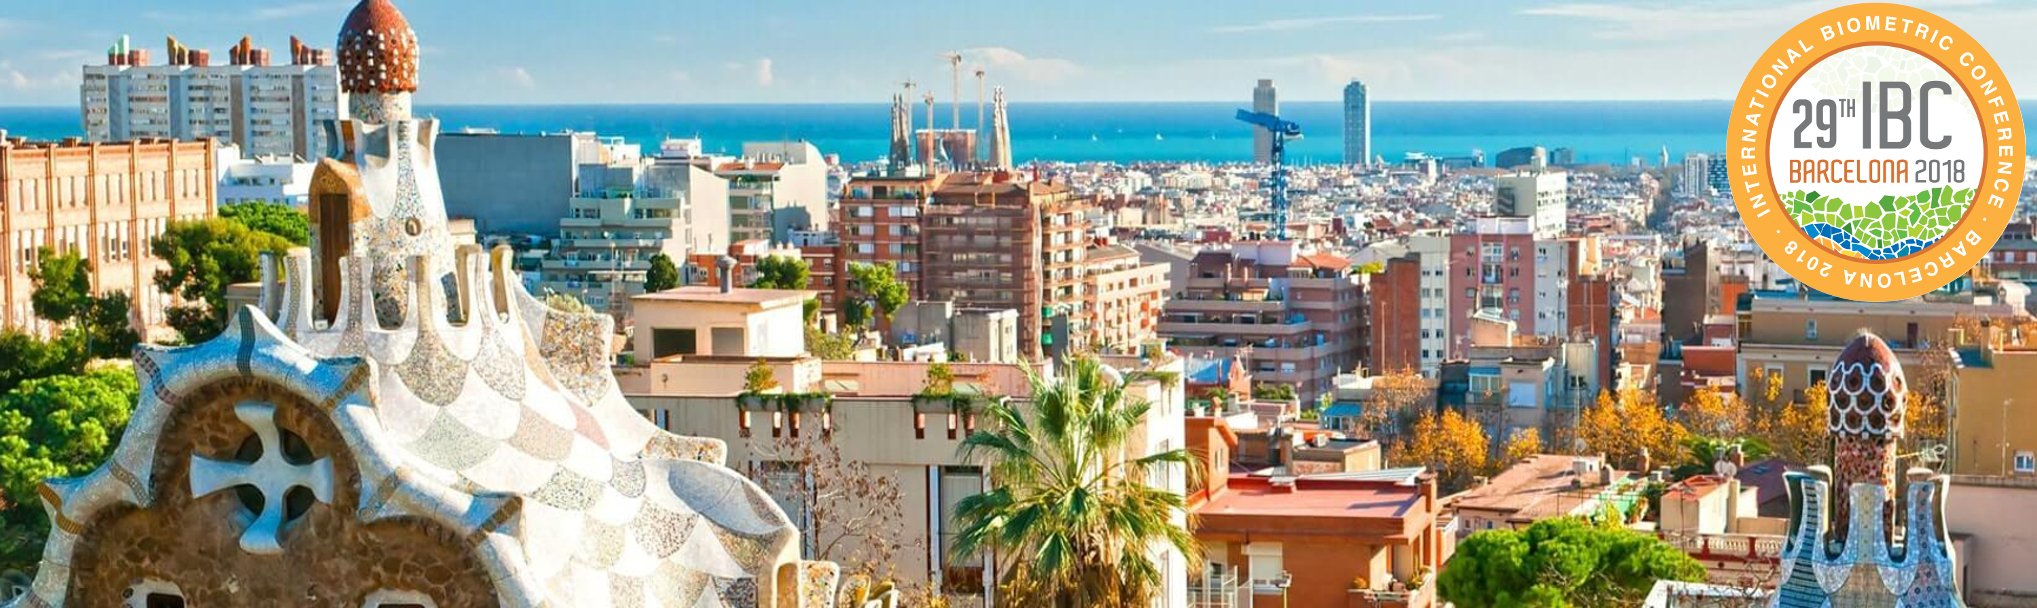
\includegraphics[width=0.9\textwidth]{./images/ibc-2018-barcelona.jpg}
	\end{center}
	
	
\end{frame}





\section*{References}
\begin{frame}\frametitle{References}
\begin{thebibliography}{9}

%\addcontentsline{toc}{chapter}{\numberline{}Bibliografía}
%
%\bibitem{cohen} J. Cohen, \emph{Statistical power analysis for the behavioral sciences} (2nd ed.). % Hillsdale,NJ: Lawrence Erlbaum, 1988.

%\bibitem{faraway} J.J. Faraway, \emph{Linear Models with R}, Chapman \& Hall/CRC, 2004.

%\bibitem{montgomery} D.C Montgomery \emph{Design and Analysis of Experiments}, John Wiley \& Sons, 2008.

%\bibitem{blog} \texttt{http://erre-que-erre-paco.blogspot.com.es/2013/04/el-codigo-body-td-font-family-sans.html}

\bibitem{Bazzocco:2015} Bazzocco, Sara. \emph{et al.} (2015) \emph{Highly Expressed Genes in Rapidly Proliferating Tumor Cells as New Targets for Colorectal Cancer Treatment}. DOI: 10.1158/1078-0432.CCR-14-2457

\bibitem{Liu:2012} Liu, Y. and Qiu, P. (2012) \emph{Integrative analysis of methylation and gene expression data in TCGA} IEEE International Workshop on Genomic Signal Processing and Statistics (GENSIPS)

\bibitem{Sanchez:2017} Sánchez-Pla, A., Ruiz de Vila, M.C:, Carmona, F., Bazzoco, S. and Arango del Corro, D. (2017). 
\emph{Integrative analysis to select genes regulated by methylation in a cancer colon study} Trends in Mathematics 2017. DOI: 10.1007/978-3-319-55639-09

\bibitem{Wilkinson:2017} Wilkinson, Leland, and Graham Wills. (2017). 
\emph{``Scagnostics Distributions''}, JCGS.

\end{thebibliography}

\end{frame}



\end{document}
